% !TeX root = main.tex
\chapter{Technological developments}\label{app:tech}

\section{Browser-based audio interface}\label{sec:browser-audio-interface}
An audio interface was developed for use in evaluating a number of different audio visualizations (see
Section~\ref{sec:study}). In order to maximise the number of people who could participate in the experiment, it was
designed to be accessible online and run in a web browser.

The latest web standards (such as HTML5) were exploited in order to ensure a smooth and consistent user experience.
This meant that some people running older browsers were unable to take part, but the standards are mature enough that
the vast majority of browsers are compatible.

\subsection{Design}\label{sec:browser-audio-interface-design}
The screenshot of the  final design of the interface is shown in Figure~\ref{fig:browser-audio-interface}, which includes of one the
training pop-ups.

\begin{figure}[ht]
  \centering
  \includegraphics[width=\textwidth]{figs/interface.png}
  \caption{Experimental test interface with training pop-up}
  \label{fig:browser-audio-interface}
\end{figure}

\paragraph{Motivation}
The goal for the design was to include all the essential features required to complete the task of finding and
selecting a segment of audio (see Section~\ref{sec:studytask}) in a way that can easily be picked up by novice
participants. Only the essential features were considered in order to make it simple and to avoid distraction.

\paragraph{Displays}
Two displays were used -- one to show an overview of the entire recording, and another showing an adjustable zoom
display. It would be possible to complete the task using only an adjustable zoom display, but it would be very
difficult to keep track of the position in the recording.

The zoom display was placed above the overview display and set to be slightly larger than the overview in order to
emphasise that the display is a magnification. The two displays were linked using two curvy lines (splines) which show
the position of the zoom display limits in the overview display.

The current position of the audio playback was signified by adding a `cursor' using a line on each display. The cursor
can be moved by clicking or dragging on either of the displays using the mouse.

Selected areas of audio are highlighted using a semi-transparent overlay which appears on both displays.  A time
`ruler' was also overlaid on both displays to give users an objective scale and a sense of the relative scale of the
displays.

\paragraph{Zoom control}
The level of zoom was controlled using two buttons at the bottom -- one to zoom in and another to zoom out. In an early
prototype, users could press these buttons as many times as they wished, but this caused confusion when maximum zoom
was reached and the button stopped doing anything. Following feedback, this was rectified by disabling and greying out
the buttons when at max/min zoom.

\paragraph{Selection}
Two methods of selecting content were implemented -- one using buttons and another using a slider. The buttons were
used to set either the in or out point of the selection to the current position of the cursor. The buttons could be
used while the audio is playing, allowing users to press a button as they hear their preferred start/end point. As the
cursor can be moved on the zoomable display, the buttons can be used to set the selection precisely.

The slider acts both as a display of where the selection is and as a method of setting or adjusting it. The slider was
located just under the overview display and has `handles' on each side which can be dragged to adjust the start and end
of the selection. After receiving feedback on a prototype, the slider was configured to update the highlight in the
displays as it is dragged, making fine adjustments easier to see.

\paragraph{Training}
Although the interface is relatively basic as far as digital audio workstations are concerned, a system was developed
to train users in the features and operation of the interface. This was done using a `pop-up tour', which is a
technique often found on web pages. It involves a series of dialog boxes which point out different parts of the
interface with some text explaining what they do. You can see an example in Figure~\ref{fig:interface}.

\subsection{Implementation}

\paragraph{Front-end}
A feature-heavy web page, such one that includes an audio/visual interface, can be slow to load and unresponsive. To
avoid this, the interface was set up as a `single-page application' which loads the content of each page dynamically
without having to reload the interface and the large Javascript libraries that it's built on.

Angular.JS\footnote{\url{https://angularjs.org}} is a Javascript web application framework which aids development of
dynamic web pages. A single-page application was implemented using its `route' and `view' features.  Its other features
were used to send responses to the database and update the cursor/selection on the visualization, amongst other things.

Bootstrap\footnote{\url{http://getbootstrap.com/}} was used to style the page and the components in it. The popularity
of Bootstrap means that this style is familiar and comfortable to most web users. Bootstrap
Tour\footnote{\url{http://bootstraptour.com/}} is a Javascript library for running `pop-up tours' on websites. This was
used to implement the training interface, as discussed in Section~\ref{sec:interfacedesign}.

\paragraph{Back-end}
A web server and database were used to serve the web pages and experimental data, and to store the results.
Node.js\footnote{\url{http://nodejs.org/}} was used to implement and expose an API for interacting with the front-end
and CouchDB\footnote{\url{http://couchdb.apache.org/}} was used as the database.

The sequence for each experiment (described in Section~\ref{sec:studysequence}) needed to be assigned to participants
evenly, so that each sequence is completed exactly once before a second participant is assigned to it. This was done by
taking the sequences that had been completed the least number of times, then choosing the sequence that had been
assigned the longest time ago (or not at all). This approach minimised the chance of more than one participant using
the same sequence. 

\paragraph{Audio playback}
Different browsers support a variety of different audio codecs and have different capabilities in terms of playback
methods. In order to maximise compatibility, SoundJS\footnote{\url{http://www.createjs.com/\#!/SoundJS}} was used to
play the audio content.

The audio content was data compressed using a lossy codec to reduce the size (and therefore loading time) of each web
page. Ogg Vorbis was used as the primary codec, with a quality setting of 2 (approx. 80kbps VBR). For browsers that
didn't support Ogg Vorbis, AAC was used with a variable bitrate of 96kbps.  The use of lossy codecs introduces some
audible artefacts. However this is not part of the experiment and it impacts every audio clip, so is not expected to
bias the results. 

\paragraph{Visualization}
The duration of each of the audio clips used in the experiment is about 5 minutes, and the interface display allows for
four levels of zoom. This produces up to $\sim$2MB of image data which, if loaded at the beginning, would negatively
impact on the loading time of the web page. To fix this, a tiling system was used where each image was cut into tiles
240 pixels wide. The displays then dynamically loaded the tiles as and when they were needed.

To ensure maximum browser compatibility and to simplify the implementation,
KineticJS\footnote{\url{http://kineticjs.com/}} was used to render the images, ruler and cursor.

\clearpage
\section{Vampeyer}\label{sec:vampeyer}
The direction of the research in this project centres around turning audio data into image data. There is already some
software that visualizes audio and audio features in a number of ways, notably Sonic Visualiser \citep{Cannam2010}.
However, the visualization algorithms are always hard-coded into the program, making prototyping of new methods
prohibitively difficult.

\subsection{Design}
A system of software was developed for visualizing audio in order to allow flexibility while maintaining consist inputs
and outputs. It was designed to expand on existing systems for audio analysis so to avoid duplication of effort and to
allow modularisation of algorithms.

The system was developed as a plugin framework with clearly defined inputs and outputs. It is based on the existing
Vamp plugin framework, developed by Queen Mary University of London \citep{Cannam2010}, which analyses audio data and
outputs frame-- or time-based features. The visualization plugin is designed to take these features and produce a
bitmap image. An outline of the system design is shown in Figure~\ref{fig:vampeyer}.

\begin{figure}[ht]
  \centering
  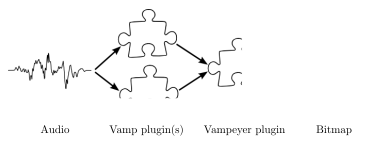
\includegraphics[width=0.8\textwidth]{figs/vampeyer.png}
  \caption{High-level system diagram of the Vampeyer visualization framework}
  \label{fig:vampeyer}
\end{figure}

The visualization plugin defines which Vamp plugin outputs it requires, including the block/step size and parameters.
At least one Vamp plugin is required, but there is no restriction of the number of different Vamp plugins that can be
used.

Both frameworks are written in C++ which allows for a fast processing time.  This is important for situations where
audio has to be processed on-the-fly, such as for exploring an archive without having to pre-process everything in it.
The plugins are compiled into shared libraries, so they can easily be distributed without users having to recompile
locally and integrated into third-party software.

\subsection{Implementation}
A C++ header file was created which implements the design.  Five data structures are also defined which define how data
should be sent and returned from the functions.

{\singlespacing
\begin{itemize}
  \item \texttt{VampParameter} is a name/value pair used to store a parameter
  \item \texttt{VampParameterList} is a vector of \texttt{VampParameter}s
  \item \texttt{VampPlugin} stores the name of a Vamp plugin along with a\\
    \texttt{VampParameterList} and the preferred block and step sizes
  \item \texttt{VampOutput} stores a \texttt{VampPlugin} and output name
  \item \texttt{VampOutputList} is a vector of \texttt{VampOutput}s
\end{itemize}
}

Two primary functions are used to define the input audio features and their conversion to a bitmap.

\begin{itemize}
  \item \texttt{getVampPlugins} returns a \texttt{VampOutputList} variable that contains a list of Vamp plugin outputs
    which must be provided as input
  \item \texttt{ARGB} takes the Vamp plugin output data as a \texttt{Vamp::FeatureSet} variable, the sample rate of the
    audio and the desired width and height. It returns a bitmap image formatted in 32-bit ARGB format (alpha, red,
    green, blue).
\end{itemize}

A number of example plugins were written to demonstrate the capabilities of this approach, and to act as useful pieces
of software in their own right.  These include a standard waveform, waveform colourised by low energy ratio (see
Section~\ref{sec:studywaveform}), waveform colourised by spectral centroid (identical to Freesound) and an MFCC grid
visualization with waveform overlay.

The plugins need to be run by a host program which reads the audio data, processes it using the Vamp plugins, sends
their output to the visualization plugin and then writes the image data. Such a program was written as a command-line
tool that can either display the image in a window or write it to disk as a PNG-encoded file. This makes it useful for
both prototyping and for back-end processing on a server, for example.

\clearpage
\section{BeatMap}\label{sec:beatmap}

\clearpage
\section{Dialogger}\label{sec:dialogger}

\texttt{https://github.com/bbc/dialogger}

\begin{figure}
\centering
  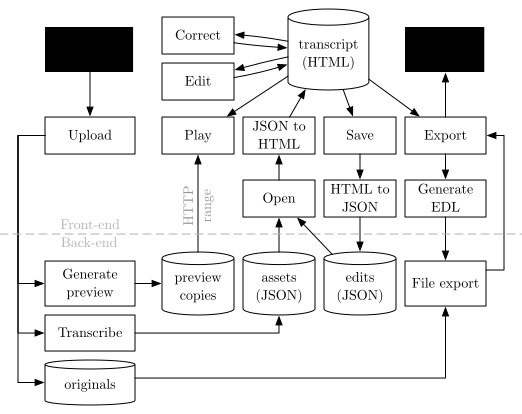
\includegraphics[width=\columnwidth]{figs/dialogger-flow-diagram.png}
  \caption{Flow diagram of the Dialogger system. Excluded components are shown in red.}
  \label{fig:dialogger-flow}
\end{figure}

Made a screen-based semantic speech editor. Here's how it works.
